\chapter[Análisis]{
  \label{chp:analisis}
  ANÁLISIS
}
\thispagestyle{numberingStyle}
\pagestyle{numberingStyle}

En este apartado se explicará, detalladamente, el análisis realizado.

\section{Análisis de requerimientos}

\subsection{Requerimientos funcionales}
A continuación se muestran los requerimientos funcionales del sistema, clasificados en distintas áreas.

\subsubsection*{Acceso a la aplicación}
\begin{itemize}
\setlength\itemsep{1pt}
\item El sistema ofrecerá la posibilidad de que un usuario se registre en la aplicación.
\item El sistema ofrecerá la posibilidad de que el usuario se identifique en el sistema. Los usuarios deben ingresar al sistema con  nombre de usuario y contraseña.
\end{itemize}

\subsubsection*{Aplicación Móvil}
\begin{itemize}
\setlength\itemsep{1pt}
\item El sistema ofrecerá la posibilidad de crear nuevas rutas.
\item El usuario podrá consultar las rutas, propias y de otros usuarios, según ciertos criterios de búsqueda.
\item El sistema permitirá a los usuarios autorizados eliminar las rutas propias que deseen.
\item El sistema permitirá a los usuarios autorizados a consultar los detalles de las rutas.
\item Para las rutas, el sistema permitirá:
	\begin{itemize}
	\item Establecer las fechas de inicio y fin.
	\item Consultar, asignar y desasignar a la ruta, los eventos disponibles en esas fechas.
	\item Consultar el itinerario por días.
	\item Modificar la hora de comienzo establecida para cada día.
	\item Consultar, añadir y eliminar lugares de interés a cada día de la ruta.
	\item Editar el modo de viaje a realizar entre diferentes lugares.
	\item Mostrar el itinerario, por días y en total, en el mapa.
	\item Habilitar y deshabilitar el sistema de geolocalización para conocer la ruta hecha en tiempo real.
	\item Consultar y comparar, el itinerario definido con el obtenido a tiempo real.
	\item Editar los permisos de la ruta.
	\end{itemize}
\end{itemize}

\subsubsection*{Aplicación Web}
\begin{itemize}
\setlength\itemsep{1pt}
\item El usuario podrá consultar las rutas existentes, propias y de otros usuarios, según ciertos criterios de búsqueda.
\item El sistema permitirá a los usuarios autorizados a consultar los detalles de las rutas.
\item El sistema permitirá a los usuarios autorizados marcar las rutas propias como privadas, con el fin de no compartirlas con los demás usuarios.
\item El sistema solo ofrecerá la posibilidad de consulta sobre los detalles de una ruta, permitiendo ver el itinerario, si tiene datos en tiempo real guardados, etc...
\item El sistema permitirá a los usuarios autorizados eliminar las rutas propias que deseen.
\end{itemize}

\subsubsection*{Administración Web}
\begin{itemize}
\setlength\itemsep{1pt}
\item El sistema solo permitirá acceso a usuarios con permisos de administración.
\item El sistema permitirá a los usuarios con dichos permisos, dar de alto nuevos usuarios.
\item El sistema permitirá las altas, bajas, modificaciones y consultas de las entidades del sistema.
	\begin{itemize}
	\item El sistema ofrecerá la posibilidad de crear, eliminar, modificar y consultar datos de usuarios.
	\item El sistema ofrecerá la posibilidad de crear, eliminar, modificar y consultar datos de rutas.
	\item El sistema ofrecerá la posibilidad de crear, eliminar, modificar y consultar datos de lugares.
	\item El sistema ofrecerá la posibilidad de crear, eliminar, modificar y consultar datos de categorías.
	\item El sistema ofrecerá la posibilidad de crear, eliminar, modificar y consultar datos de eventos.
	\end{itemize}

\end{itemize}

\subsubsection*{Seguridad}
\begin{itemize}
\setlength\itemsep{1pt}
\item El sistema ofrecerá la posibilidad de que el usuario modifique sus datos de acceso al sistema.
\item El sistema solo permitirá acciones correctamente autenticadas, exceptuando las de acceso a la aplicación.
\item Los usuarios de la aplicación solo podrán modificar los datos a los que el usuario esté autorizado. Un usuario no podrá modificar la información de los recursos de los que no es propietario.
\item Los intercambios de datos que realice el sistema a través de internet, serán mediante el uso del protocolo encriptado https.
\end{itemize}


\subsection{Requerimientos no funcionales}
\subsubsection*{Rendimiento}
\subsubsection*{Disponibilidad}
\subsubsection*{Estabilidad}
\subsubsection*{Escalabilidad}




\section{Modelo de casos de uso}

\subsection{Actores del sistema}

\subsection{Diagrama de casos de uso}



\begin{figure}[t!]
Diagrama Casos de Uso Aplicación Móvil.

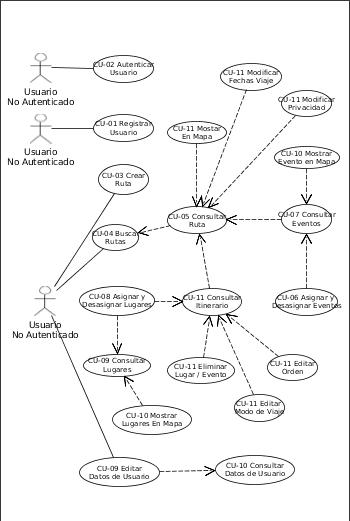
\includegraphics[
   keepaspectratio=true
]{usecase-app-movil.jpg}
\caption{Ssadsadsad}
\end{figure}










\newpage
\subsection{Especificación casos de uso}


\newpage
\subsubsection*{Autenticar Usuario}
\begin{longtable}{| p{4cm} | p{10cm} |}
\endfirsthead
\multicolumn{2}{c}{\textit{Continúa de la página anterior}}\\[12pt]
\hline
\endhead
\hline
\multicolumn{2}{c}{\textit{Continúa en la siguiente página}} \\
\endfoot
\hline
\caption{Caso de Uso: Autenticar Usuario}\label{fig:1}\\
\endlastfoot


\hline
\multicolumn{2}{|c|}{\textbf{CU$<$01$>$ Autenticar Usuario}} \\

\hline
\textbf{Descripción} &
El usuario se identifica introduciendo las credenciales de acceso en el sistema \\

\hline
\textbf{Actores} &
Usuario\newline
Administrador\newline
Moderador\\

\hline
\textbf{Precondiciones} &
N/A\\

\hline
\textbf{Secuencia Normal} &\mbox{}\par\vspace{-\baselineskip}
\begin{enumerate}[leftmargin=0.7cm, topsep=0.1cm]
\item El usuario introduce sus credenciales en la ventana de login. 
\item El usuario pulsa el botón de \textit{Acceder}.
\item El sistema valida las credenciales.
\item El usuario accede a la aplicación.
\end{enumerate}\\

\hline
\textbf{Excepciones} &\mbox{}\par\vspace{-\baselineskip}
\begin{enumerate}[leftmargin=0.9cm, topsep=0.1cm]
\item[3a.] Los datos introducidos no son correctos.
	\begin{itemize}
	\item[1.] El usuario vuelve a introducir las credenciales.
	\end{itemize}

\end{enumerate}\\

\hline
\textbf{Postcondiciones} & 
El usuario queda autenticado en el sistema\\
\hline
\end{longtable}




\newpage
\subsubsection*{Registrar Usuario}
\begin{longtable}{| p{4cm} | p{10cm} |}
\endfirsthead
\multicolumn{2}{c}{\textit{Continúa de la página anterior}}\\[12pt]
\hline
\endhead
\hline
\multicolumn{2}{c}{\textit{Continúa en la siguiente página}} \\
\endfoot
\hline
\caption{Caso de Uso: Registrar Usuario}\label{fig:1}\\
\endlastfoot


\hline
\multicolumn{2}{|c|}{\textbf{CU$<$02$>$ Registrar Usuario}} \\

\hline
\textbf{Descripción} &
El usuario introduce los datos para darse de alta en la aplicación. \\

\hline
\textbf{Actores} &
Usuario\\


\hline
\textbf{Precondiciones} &
N/A\\

\hline
\textbf{Secuencia Normal} &\mbox{}\par\vspace{-\baselineskip}
\begin{enumerate}[leftmargin=0.7cm, topsep=0.1cm]
\item El usuario selecciona la opción de registrarse.
\item El sistema muestra un formulario indicando los campos necesarios para realizar el registro.
\item El usuario rellena los campos y pulsa el botón de \textit{Registrarse}.
\item El sistema valida los datos introducidos por el usuario.
\item El usuario accede a la aplicación.
\end{enumerate}\\

\hline
\textbf{Excepciones} &\mbox{}\par\vspace{-\baselineskip}
\begin{enumerate}[leftmargin=0.9cm, topsep=0.1cm]
\item[3a.] El usuario pulsa el botón de \textit{Cancelar}.
	\begin{itemize}
	\item[1.] El sistema cancela el registro y redirige al usuario a la pantalla de login.
	\item[2.] Implementa CU-$<$01$>$ Autenticar Usuario
	\end{itemize}
\item[3a.] Los datos introducidos por el usuario no son válidos.
	\begin{itemize}
	\item[1.] El sistema muestra un mensaje de error e invita al usuario a volver a introducir los datos. (Regreso al paso 2)
	\end{itemize}

\end{enumerate}\\

\hline
\textbf{Postcondiciones} & 
El usuario queda registrado y autenticado en el sistema\\
\hline
\end{longtable}